\documentclass[1p]{elsarticle_modified}
%\bibliographystyle{elsarticle-num}

%\usepackage[colorlinks]{hyperref}
%\usepackage{abbrmath_seonhwa} %\Abb, \Ascr, \Acal ,\Abf, \Afrak
\usepackage{amsfonts}
\usepackage{amssymb}
\usepackage{amsmath}
\usepackage{amsthm}
\usepackage{scalefnt}
\usepackage{amsbsy}
\usepackage{kotex}
\usepackage{caption}
\usepackage{subfig}
\usepackage{color}
\usepackage{graphicx}
\usepackage{xcolor} %% white, black, red, green, blue, cyan, magenta, yellow
\usepackage{float}
\usepackage{setspace}
\usepackage{hyperref}

\usepackage{tikz}
\usetikzlibrary{arrows}

\usepackage{multirow}
\usepackage{array} % fixed length table
\usepackage{hhline}

%%%%%%%%%%%%%%%%%%%%%
\makeatletter
\renewcommand*\env@matrix[1][\arraystretch]{%
	\edef\arraystretch{#1}%
	\hskip -\arraycolsep
	\let\@ifnextchar\new@ifnextchar
	\array{*\c@MaxMatrixCols c}}
\makeatother %https://tex.stackexchange.com/questions/14071/how-can-i-increase-the-line-spacing-in-a-matrix
%%%%%%%%%%%%%%%

\usepackage[normalem]{ulem}

\newcommand{\msout}[1]{\ifmmode\text{\sout{\ensuremath{#1}}}\else\sout{#1}\fi}
%SOURCE: \msout is \stkout macro in https://tex.stackexchange.com/questions/20609/strikeout-in-math-mode

\newcommand{\cancel}[1]{
	\ifmmode
	{\color{red}\msout{#1}}
	\else
	{\color{red}\sout{#1}}
	\fi
}

\newcommand{\add}[1]{
	{\color{blue}\uwave{#1}}
}

\newcommand{\replace}[2]{
	\ifmmode
	{\color{red}\msout{#1}}{\color{blue}\uwave{#2}}
	\else
	{\color{red}\sout{#1}}{\color{blue}\uwave{#2}}
	\fi
}

\newcommand{\Sol}{\mathcal{S}} %segment
\newcommand{\D}{D} %diagram
\newcommand{\A}{\mathcal{A}} %arc


%%%%%%%%%%%%%%%%%%%%%%%%%%%%%5 test

\def\sl{\operatorname{\textup{SL}}(2,\Cbb)}
\def\psl{\operatorname{\textup{PSL}}(2,\Cbb)}
\def\quan{\mkern 1mu \triangleright \mkern 1mu}

\theoremstyle{definition}
\newtheorem{thm}{Theorem}[section]
\newtheorem{prop}[thm]{Proposition}
\newtheorem{lem}[thm]{Lemma}
\newtheorem{ques}[thm]{Question}
\newtheorem{cor}[thm]{Corollary}
\newtheorem{defn}[thm]{Definition}
\newtheorem{exam}[thm]{Example}
\newtheorem{rmk}[thm]{Remark}
\newtheorem{alg}[thm]{Algorithm}

\newcommand{\I}{\sqrt{-1}}
\begin{document}

%\begin{frontmatter}
%
%\title{Boundary parabolic representations of knots up to 8 crossings}
%
%%% Group authors per affiliation:
%\author{Yunhi Cho} 
%\address{Department of Mathematics, University of Seoul, Seoul, Korea}
%\ead{yhcho@uos.ac.kr}
%
%
%\author{Seonhwa Kim} %\fnref{s_kim}}
%\address{Center for Geometry and Physics, Institute for Basic Science, Pohang, 37673, Korea}
%\ead{ryeona17@ibs.re.kr}
%
%\author{Hyuk Kim}
%\address{Department of Mathematical Sciences, Seoul National University, Seoul 08826, Korea}
%\ead{hyukkim@snu.ac.kr}
%
%\author{Seokbeom Yoon}
%\address{Department of Mathematical Sciences, Seoul National University, Seoul, 08826,  Korea}
%\ead{sbyoon15@snu.ac.kr}
%
%\begin{abstract}
%We find all boundary parabolic representation of knots up to 8 crossings.
%
%\end{abstract}
%\begin{keyword}
%    \MSC[2010] 57M25 
%\end{keyword}
%
%\end{frontmatter}

%\linenumbers
%\tableofcontents
%
\newcommand\colored[1]{\textcolor{white}{\rule[-0.35ex]{0.8em}{1.4ex}}\kern-0.8em\color{red} #1}%
%\newcommand\colored[1]{\textcolor{white}{ #1}\kern-2.17ex	\textcolor{white}{ #1}\kern-1.81ex	\textcolor{white}{ #1}\kern-2.15ex\color{red}#1	}

{\Large $\underline{12n_{0380}~(K12n_{0380})}$}

\setlength{\tabcolsep}{10pt}
\renewcommand{\arraystretch}{1.6}
\vspace{1cm}\begin{tabular}{m{100pt}>{\centering\arraybackslash}m{274pt}}
\multirow{5}{120pt}{
	\centering
	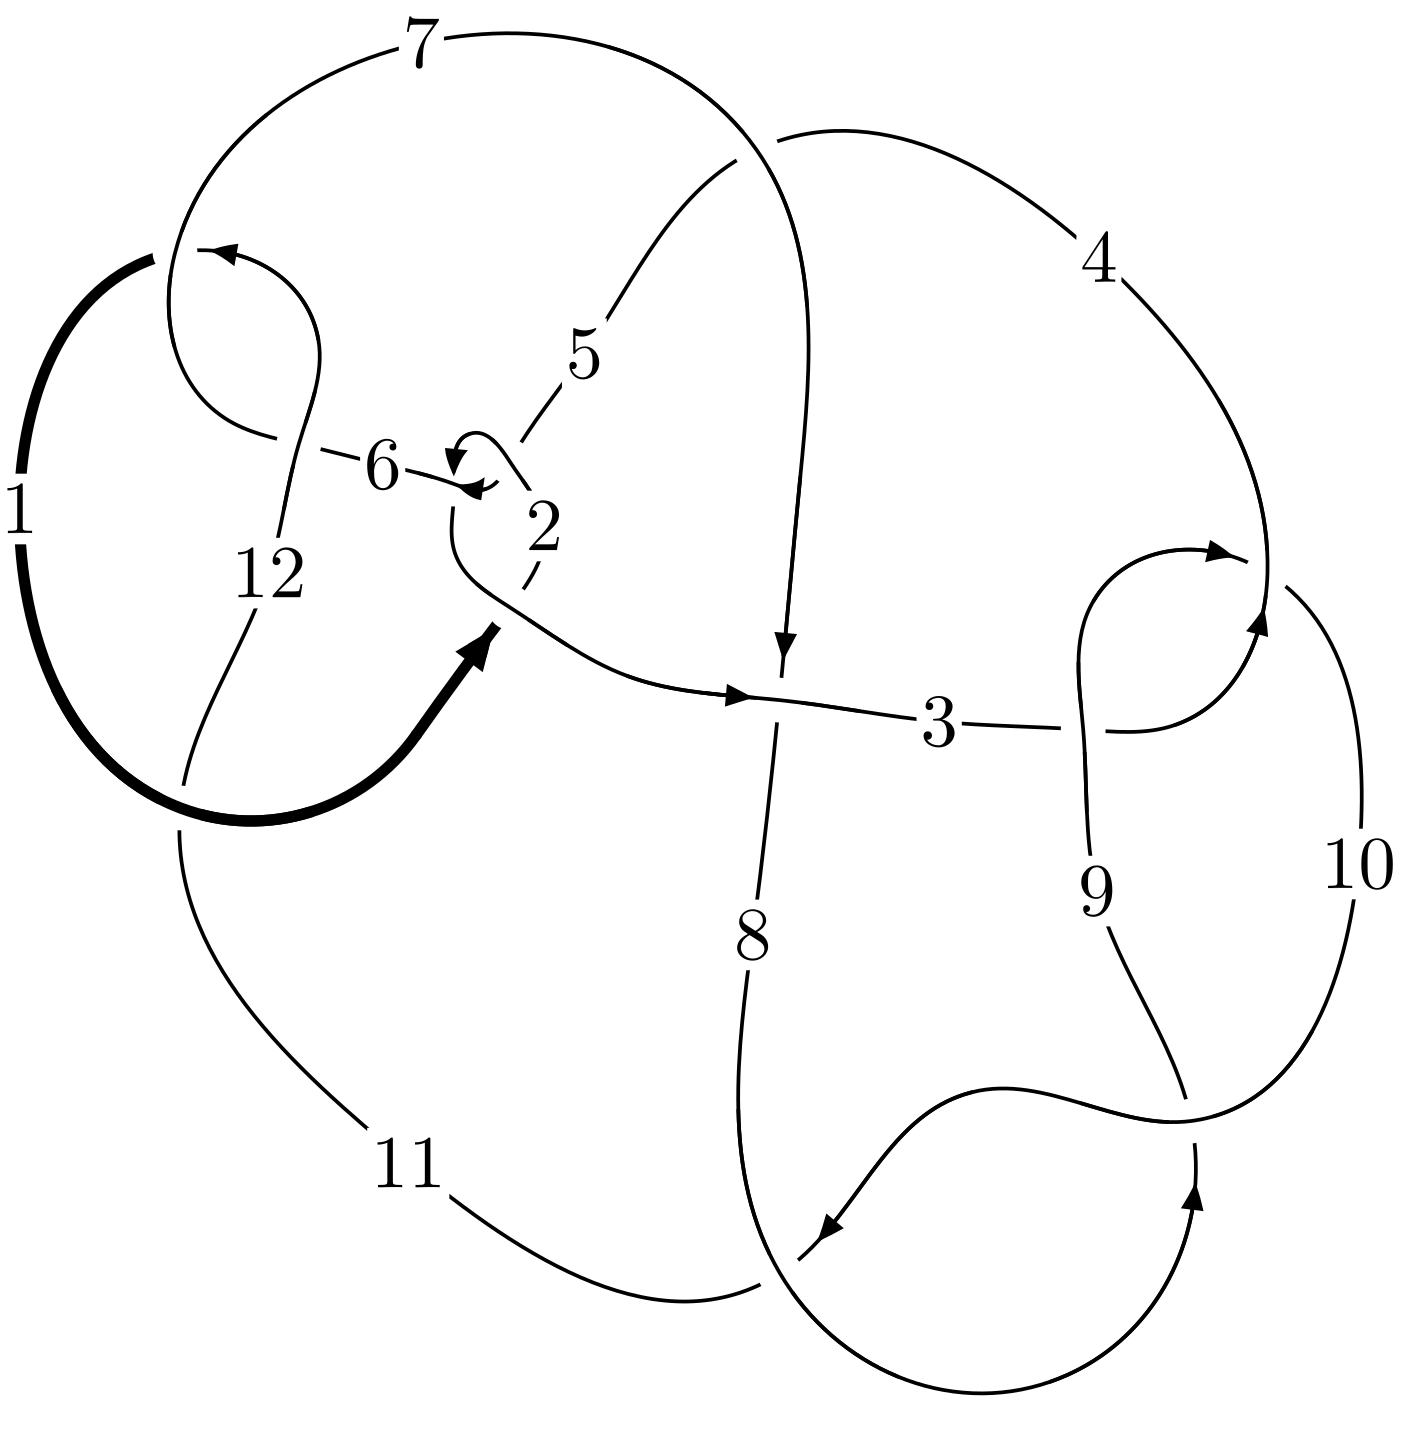
\includegraphics[width=112pt]{../../../GIT/diagram.site/Diagrams/png/2469_12n_0380.png}\\
\ \ \ A knot diagram\footnotemark}&
\allowdisplaybreaks
\textbf{Linearized knot diagam} \\
\cline{2-2}
 &
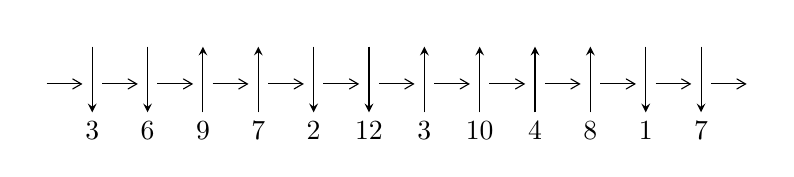
\begin{tikzpicture}[x=20pt, y=17pt]
	% nodes
	\node (C0) at (0, 0) {};
	\node (C1) at (1, 0) {};
	\node (C1U) at (1, +1) {};
	\node (C1D) at (1, -1) {3};

	\node (C2) at (2, 0) {};
	\node (C2U) at (2, +1) {};
	\node (C2D) at (2, -1) {6};

	\node (C3) at (3, 0) {};
	\node (C3U) at (3, +1) {};
	\node (C3D) at (3, -1) {9};

	\node (C4) at (4, 0) {};
	\node (C4U) at (4, +1) {};
	\node (C4D) at (4, -1) {7};

	\node (C5) at (5, 0) {};
	\node (C5U) at (5, +1) {};
	\node (C5D) at (5, -1) {2};

	\node (C6) at (6, 0) {};
	\node (C6U) at (6, +1) {};
	\node (C6D) at (6, -1) {12};

	\node (C7) at (7, 0) {};
	\node (C7U) at (7, +1) {};
	\node (C7D) at (7, -1) {3};

	\node (C8) at (8, 0) {};
	\node (C8U) at (8, +1) {};
	\node (C8D) at (8, -1) {10};

	\node (C9) at (9, 0) {};
	\node (C9U) at (9, +1) {};
	\node (C9D) at (9, -1) {4};

	\node (C10) at (10, 0) {};
	\node (C10U) at (10, +1) {};
	\node (C10D) at (10, -1) {8};

	\node (C11) at (11, 0) {};
	\node (C11U) at (11, +1) {};
	\node (C11D) at (11, -1) {1};

	\node (C12) at (12, 0) {};
	\node (C12U) at (12, +1) {};
	\node (C12D) at (12, -1) {7};
	\node (C13) at (13, 0) {};

	% arrows
	\draw[->,>={angle 60}]
	(C0) edge (C1) (C1) edge (C2) (C2) edge (C3) (C3) edge (C4) (C4) edge (C5) (C5) edge (C6) (C6) edge (C7) (C7) edge (C8) (C8) edge (C9) (C9) edge (C10) (C10) edge (C11) (C11) edge (C12) (C12) edge (C13) ;	\draw[->,>=stealth]
	(C1U) edge (C1D) (C2U) edge (C2D) (C3D) edge (C3U) (C4D) edge (C4U) (C5U) edge (C5D) (C6U) edge (C6D) (C7D) edge (C7U) (C8D) edge (C8U) (C9D) edge (C9U) (C10D) edge (C10U) (C11U) edge (C11D) (C12U) edge (C12D) ;
	\end{tikzpicture} \\
\hhline{~~} \\& 
\textbf{Solving Sequence} \\ \cline{2-2} 
 &
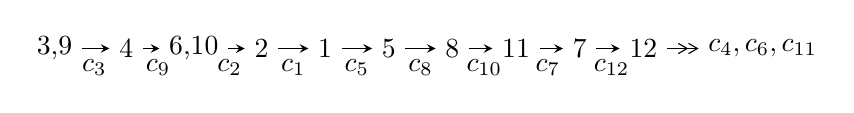
\begin{tikzpicture}[x=23pt, y=7pt]
	% node
	\node (A0) at (-1/8, 0) {3,9};
	\node (A1) at (1, 0) {4};
	\node (A2) at (33/16, 0) {6,10};
	\node (A3) at (25/8, 0) {2};
	\node (A4) at (33/8, 0) {1};
	\node (A5) at (41/8, 0) {5};
	\node (A6) at (49/8, 0) {8};
	\node (A7) at (57/8, 0) {11};
	\node (A8) at (65/8, 0) {7};
	\node (A9) at (73/8, 0) {12};
	\node (C1) at (1/2, -1) {$c_{3}$};
	\node (C2) at (3/2, -1) {$c_{9}$};
	\node (C3) at (21/8, -1) {$c_{2}$};
	\node (C4) at (29/8, -1) {$c_{1}$};
	\node (C5) at (37/8, -1) {$c_{5}$};
	\node (C6) at (45/8, -1) {$c_{8}$};
	\node (C7) at (53/8, -1) {$c_{10}$};
	\node (C8) at (61/8, -1) {$c_{7}$};
	\node (C9) at (69/8, -1) {$c_{12}$};
	\node (A10) at (11, 0) {$c_{4},c_{6},c_{11}$};

	% edge
	\draw[->,>=stealth]	
	(A0) edge (A1) (A1) edge (A2) (A2) edge (A3) (A3) edge (A4) (A4) edge (A5) (A5) edge (A6) (A6) edge (A7) (A7) edge (A8) (A8) edge (A9) ;
	\draw[->>,>={angle 60}]	
	(A9) edge (A10);
\end{tikzpicture} \\ 

\end{tabular} \\

\footnotetext{
The image of knot diagram is generated by the software ``\textbf{Draw programme}" developed by Andrew Bartholomew(\url{http://www.layer8.co.uk/maths/draw/index.htm\#Running-draw}), where we modified some parts for our purpose(\url{https://github.com/CATsTAILs/LinksPainter}).
}\phantom \\ \newline 
\centering \textbf{Ideals for irreducible components\footnotemark of $X_{\text{par}}$} 
 
\begin{align*}
I^u_{1}&=\langle 
u^{24}+2 u^{23}+\cdots+b-1,\;- u^{24}- u^{23}+\cdots+2 a-2,\;u^{25}+3 u^{24}+\cdots-4 u-2\rangle \\
I^u_{2}&=\langle 
-36 u^{11} a+71 u^{11}+\cdots+286 a-731,\;-2 u^{11} a+2 u^{10} a+\cdots-4 a-1,\\
\phantom{I^u_{2}}&\phantom{= \langle  }u^{12}-2 u^{10}+u^9+4 u^8- u^7-3 u^6+3 u^5+3 u^4- u^3- u^2+2 u+1\rangle \\
I^u_{3}&=\langle 
b+1,\;- u^3+2 u^2+2 a+u-2,\;u^4- u^2+2\rangle \\
I^u_{4}&=\langle 
b-1,\;a- u,\;u^4+1\rangle \\
I^u_{5}&=\langle 
b,\;a+1,\;u-1\rangle \\
I^u_{6}&=\langle 
b+1,\;a-2,\;u-1\rangle \\
I^u_{7}&=\langle 
b+1,\;a-3,\;u-1\rangle \\
I^u_{8}&=\langle 
b+1,\;a-1,\;u+1\rangle \\
\\
I^v_{1}&=\langle 
a,\;b-1,\;v+1\rangle \\
\end{align*}
\raggedright * 9 irreducible components of $\dim_{\mathbb{C}}=0$, with total 62 representations.\\
\footnotetext{All coefficients of polynomials are rational numbers. But the coefficients are sometimes approximated in decimal forms when there is not enough margin.}
\newpage
\renewcommand{\arraystretch}{1}
\centering \section*{I. $I^u_{1}= \langle u^{24}+2 u^{23}+\cdots+b-1,\;- u^{24}- u^{23}+\cdots+2 a-2,\;u^{25}+3 u^{24}+\cdots-4 u-2 \rangle$}
\flushleft \textbf{(i) Arc colorings}\\
\begin{tabular}{m{7pt} m{180pt} m{7pt} m{180pt} }
\flushright $a_{3}=$&$\begin{pmatrix}1\\0\end{pmatrix}$ \\
\flushright $a_{9}=$&$\begin{pmatrix}0\\u\end{pmatrix}$ \\
\flushright $a_{4}=$&$\begin{pmatrix}1\\- u^2\end{pmatrix}$ \\
\flushright $a_{6}=$&$\begin{pmatrix}\frac{1}{2} u^{24}+\frac{1}{2} u^{23}+\cdots+u^2+1\\- u^{24}-2 u^{23}+\cdots+2 u+1\end{pmatrix}$ \\
\flushright $a_{10}=$&$\begin{pmatrix}u\\- u^3+u\end{pmatrix}$ \\
\flushright $a_{2}=$&$\begin{pmatrix}\frac{1}{2} u^{24}+\frac{5}{2} u^{23}+\cdots-3 u-2\\- u^{23}- u^{22}+\cdots+2 u+1\end{pmatrix}$ \\
\flushright $a_{1}=$&$\begin{pmatrix}\frac{1}{2} u^{24}+\frac{3}{2} u^{23}+\cdots- u-1\\- u^{23}- u^{22}+\cdots+2 u+1\end{pmatrix}$ \\
\flushright $a_{5}=$&$\begin{pmatrix}- u^{12}+u^{10}-3 u^8+2 u^6-2 u^4+u^2+1\\u^{12}-2 u^{10}+4 u^8-4 u^6+3 u^4-2 u^2\end{pmatrix}$ \\
\flushright $a_{8}=$&$\begin{pmatrix}- u^3\\u^5- u^3+u\end{pmatrix}$ \\
\flushright $a_{11}=$&$\begin{pmatrix}u^5+u\\- u^7+u^5-2 u^3+u\end{pmatrix}$ \\
\flushright $a_{7}=$&$\begin{pmatrix}- u^5- u\\u^5- u^3+u\end{pmatrix}$ \\
\flushright $a_{12}=$&$\begin{pmatrix}-\frac{1}{2} u^{24}-\frac{5}{2} u^{23}+\cdots+4 u+3\\u^{23}+u^{22}+\cdots- u-1\end{pmatrix}$\\&\end{tabular}
\flushleft \textbf{(ii) Obstruction class $= -1$}\\~\\
\flushleft \textbf{(iii) Cusp Shapes $= -2 u^{24}+10 u^{22}+6 u^{21}-30 u^{20}-24 u^{19}+54 u^{18}+64 u^{17}-72 u^{16}-112 u^{15}+54 u^{14}+150 u^{13}-12 u^{12}-142 u^{11}-42 u^{10}+100 u^9+66 u^8-34 u^7-56 u^6-6 u^5+22 u^4+18 u^3-2 u-4$}\\~\\
\newpage\renewcommand{\arraystretch}{1}
\flushleft \textbf{(iv) u-Polynomials at the component}\newline \\
\begin{tabular}{m{50pt}|m{274pt}}
Crossings & \hspace{64pt}u-Polynomials at each crossing \\
\hline $$\begin{aligned}c_{1},c_{11}\end{aligned}$$&$\begin{aligned}
&u^{25}+5 u^{24}+\cdots+11 u+1
\end{aligned}$\\
\hline $$\begin{aligned}c_{2},c_{5},c_{6}\\c_{12}\end{aligned}$$&$\begin{aligned}
&u^{25}+u^{24}+\cdots+u-1
\end{aligned}$\\
\hline $$\begin{aligned}c_{3},c_{9}\end{aligned}$$&$\begin{aligned}
&u^{25}+3 u^{24}+\cdots-4 u-2
\end{aligned}$\\
\hline $$\begin{aligned}c_{4}\end{aligned}$$&$\begin{aligned}
&u^{25}+21 u^{24}+\cdots+13332 u+2962
\end{aligned}$\\
\hline $$\begin{aligned}c_{7}\end{aligned}$$&$\begin{aligned}
&u^{25}-3 u^{24}+\cdots-92 u-26
\end{aligned}$\\
\hline $$\begin{aligned}c_{8},c_{10}\end{aligned}$$&$\begin{aligned}
&u^{25}-9 u^{24}+\cdots-8 u-4
\end{aligned}$\\
\hline
\end{tabular}\\~\\
\newpage\renewcommand{\arraystretch}{1}
\flushleft \textbf{(v) Riley Polynomials at the component}\newline \\
\begin{tabular}{m{50pt}|m{274pt}}
Crossings & \hspace{64pt}Riley Polynomials at each crossing \\
\hline $$\begin{aligned}c_{1},c_{11}\end{aligned}$$&$\begin{aligned}
&y^{25}+43 y^{24}+\cdots+11 y-1
\end{aligned}$\\
\hline $$\begin{aligned}c_{2},c_{5},c_{6}\\c_{12}\end{aligned}$$&$\begin{aligned}
&y^{25}-5 y^{24}+\cdots+11 y-1
\end{aligned}$\\
\hline $$\begin{aligned}c_{3},c_{9}\end{aligned}$$&$\begin{aligned}
&y^{25}-9 y^{24}+\cdots-8 y-4
\end{aligned}$\\
\hline $$\begin{aligned}c_{4}\end{aligned}$$&$\begin{aligned}
&y^{25}-33 y^{24}+\cdots-42476552 y-8773444
\end{aligned}$\\
\hline $$\begin{aligned}c_{7}\end{aligned}$$&$\begin{aligned}
&y^{25}-21 y^{24}+\cdots-4952 y-676
\end{aligned}$\\
\hline $$\begin{aligned}c_{8},c_{10}\end{aligned}$$&$\begin{aligned}
&y^{25}+15 y^{24}+\cdots+320 y-16
\end{aligned}$\\
\hline
\end{tabular}\\~\\
\newpage\flushleft \textbf{(vi) Complex Volumes and Cusp Shapes}
$$\begin{array}{c|c|c}  
\text{Solutions to }I^u_{1}& \I (\text{vol} + \sqrt{-1}CS) & \text{Cusp shape}\\
 \hline 
\begin{aligned}
u &= -0.980316 + 0.233102 I \\
a &= \phantom{-}0.44130 + 2.47602 I \\
b &= -0.622808 - 0.762022 I\end{aligned}
 & \phantom{-}2.82058 - 3.81422 I & \phantom{-}4.98039 + 6.61368 I \\ \hline\begin{aligned}
u &= -0.980316 - 0.233102 I \\
a &= \phantom{-}0.44130 - 2.47602 I \\
b &= -0.622808 + 0.762022 I\end{aligned}
 & \phantom{-}2.82058 + 3.81422 I & \phantom{-}4.98039 - 6.61368 I \\ \hline\begin{aligned}
u &= -0.568077 + 0.832369 I \\
a &= \phantom{-}0.51973 - 1.50739 I \\
b &= -1.13721 + 0.86526 I\end{aligned}
 & \phantom{-}4.15791 + 8.74016 I & -1.84068 - 4.40634 I \\ \hline\begin{aligned}
u &= -0.568077 - 0.832369 I \\
a &= \phantom{-}0.51973 + 1.50739 I \\
b &= -1.13721 - 0.86526 I\end{aligned}
 & \phantom{-}4.15791 - 8.74016 I & -1.84068 + 4.40634 I \\ \hline\begin{aligned}
u &= -0.733592 + 0.747057 I \\
a &= \phantom{-}0.337972 - 0.198014 I \\
b &= \phantom{-}0.611523 + 0.222308 I\end{aligned}
 & -3.30756 - 0.71712 I & -2.44059 + 3.90523 I \\ \hline\begin{aligned}
u &= -0.733592 - 0.747057 I \\
a &= \phantom{-}0.337972 + 0.198014 I \\
b &= \phantom{-}0.611523 - 0.222308 I\end{aligned}
 & -3.30756 + 0.71712 I & -2.44059 - 3.90523 I \\ \hline\begin{aligned}
u &= \phantom{-}0.932488 + 0.483370 I \\
a &= \phantom{-}0.96761 + 1.60037 I \\
b &= -0.206915 - 0.805921 I\end{aligned}
 & \phantom{-}1.59893 + 1.80276 I & \phantom{-}4.99535 - 2.09686 I \\ \hline\begin{aligned}
u &= \phantom{-}0.932488 - 0.483370 I \\
a &= \phantom{-}0.96761 - 1.60037 I \\
b &= -0.206915 + 0.805921 I\end{aligned}
 & \phantom{-}1.59893 - 1.80276 I & \phantom{-}4.99535 + 2.09686 I \\ \hline\begin{aligned}
u &= \phantom{-}0.932840\phantom{ +0.000000I} \\
a &= \phantom{-}0.687051\phantom{ +0.000000I} \\
b &= -0.498290\phantom{ +0.000000I}\end{aligned}
 & \phantom{-}1.77401\phantom{ +0.000000I} & \phantom{-}4.83650\phantom{ +0.000000I} \\ \hline\begin{aligned}
u &= \phantom{-}0.764755 + 0.774203 I \\
a &= \phantom{-}0.171446 - 0.325902 I \\
b &= \phantom{-}0.784319 + 0.533336 I\end{aligned}
 & -3.51376 - 2.47052 I & -3.49276 + 4.45848 I\\
 \hline 
 \end{array}$$\newpage$$\begin{array}{c|c|c}  
\text{Solutions to }I^u_{1}& \I (\text{vol} + \sqrt{-1}CS) & \text{Cusp shape}\\
 \hline 
\begin{aligned}
u &= \phantom{-}0.764755 - 0.774203 I \\
a &= \phantom{-}0.171446 + 0.325902 I \\
b &= \phantom{-}0.784319 - 0.533336 I\end{aligned}
 & -3.51376 + 2.47052 I & -3.49276 - 4.45848 I \\ \hline\begin{aligned}
u &= -0.437237 + 0.783767 I \\
a &= \phantom{-}0.49146 + 1.67035 I \\
b &= -1.037150 - 0.927401 I\end{aligned}
 & \phantom{-}4.93859 - 5.35756 I & -1.01874 + 4.42089 I \\ \hline\begin{aligned}
u &= -0.437237 - 0.783767 I \\
a &= \phantom{-}0.49146 - 1.67035 I \\
b &= -1.037150 + 0.927401 I\end{aligned}
 & \phantom{-}4.93859 + 5.35756 I & -1.01874 - 4.42089 I \\ \hline\begin{aligned}
u &= \phantom{-}1.156340 + 0.047910 I \\
a &= -2.12651 + 3.13266 I \\
b &= \phantom{-}1.12099 - 0.93923 I\end{aligned}
 & \phantom{-}10.42970 + 7.39157 I & \phantom{-}4.47957 - 4.57784 I \\ \hline\begin{aligned}
u &= \phantom{-}1.156340 - 0.047910 I \\
a &= -2.12651 - 3.13266 I \\
b &= \phantom{-}1.12099 + 0.93923 I\end{aligned}
 & \phantom{-}10.42970 - 7.39157 I & \phantom{-}4.47957 + 4.57784 I \\ \hline\begin{aligned}
u &= -0.970077 + 0.698318 I \\
a &= \phantom{-}0.166009 + 0.595943 I \\
b &= -0.620681 + 0.170359 I\end{aligned}
 & -2.58593 - 4.79128 I & -0.37722 + 2.00234 I \\ \hline\begin{aligned}
u &= -0.970077 - 0.698318 I \\
a &= \phantom{-}0.166009 - 0.595943 I \\
b &= -0.620681 - 0.170359 I\end{aligned}
 & -2.58593 + 4.79128 I & -0.37722 - 2.00234 I \\ \hline\begin{aligned}
u &= \phantom{-}0.951621 + 0.731482 I \\
a &= -0.63483 - 1.61897 I \\
b &= -0.831342 + 0.569410 I\end{aligned}
 & -2.94773 + 8.15802 I & -2.49516 - 9.64578 I \\ \hline\begin{aligned}
u &= \phantom{-}0.951621 - 0.731482 I \\
a &= -0.63483 + 1.61897 I \\
b &= -0.831342 - 0.569410 I\end{aligned}
 & -2.94773 - 8.15802 I & -2.49516 + 9.64578 I \\ \hline\begin{aligned}
u &= -1.076120 + 0.616232 I \\
a &= -2.32949 + 1.21588 I \\
b &= \phantom{-}1.02897 - 0.98641 I\end{aligned}
 & \phantom{-}6.80687 + 0.12880 I & \phantom{-}1.81794 + 0.42247 I\\
 \hline 
 \end{array}$$\newpage$$\begin{array}{c|c|c}  
\text{Solutions to }I^u_{1}& \I (\text{vol} + \sqrt{-1}CS) & \text{Cusp shape}\\
 \hline 
\begin{aligned}
u &= -1.076120 - 0.616232 I \\
a &= -2.32949 - 1.21588 I \\
b &= \phantom{-}1.02897 + 0.98641 I\end{aligned}
 & \phantom{-}6.80687 - 0.12880 I & \phantom{-}1.81794 - 0.42247 I \\ \hline\begin{aligned}
u &= -1.066850 + 0.683933 I \\
a &= -0.18246 - 3.26046 I \\
b &= \phantom{-}1.16937 + 0.87177 I\end{aligned}
 & \phantom{-}5.6578 - 14.4091 I & \phantom{-}0.10967 + 8.76133 I \\ \hline\begin{aligned}
u &= -1.066850 - 0.683933 I \\
a &= -0.18246 + 3.26046 I \\
b &= \phantom{-}1.16937 - 0.87177 I\end{aligned}
 & \phantom{-}5.6578 + 14.4091 I & \phantom{-}0.10967 - 8.76133 I \\ \hline\begin{aligned}
u &= \phantom{-}0.060646 + 0.510945 I \\
a &= \phantom{-}0.334239 + 0.498112 I \\
b &= \phantom{-}0.490067 - 0.520637 I\end{aligned}
 & -0.268317 + 1.373590 I & -2.13600 - 4.81420 I \\ \hline\begin{aligned}
u &= \phantom{-}0.060646 - 0.510945 I \\
a &= \phantom{-}0.334239 - 0.498112 I \\
b &= \phantom{-}0.490067 + 0.520637 I\end{aligned}
 & -0.268317 - 1.373590 I & -2.13600 + 4.81420 I\\
 \hline 
 \end{array}$$\newpage\newpage\renewcommand{\arraystretch}{1}
\centering \section*{II. $I^u_{2}= \langle -36 u^{11} a+71 u^{11}+\cdots+286 a-731,\;-2 u^{11} a+2 u^{10} a+\cdots-4 a-1,\;u^{12}-2 u^{10}+\cdots+2 u+1 \rangle$}
\flushleft \textbf{(i) Arc colorings}\\
\begin{tabular}{m{7pt} m{180pt} m{7pt} m{180pt} }
\flushright $a_{3}=$&$\begin{pmatrix}1\\0\end{pmatrix}$ \\
\flushright $a_{9}=$&$\begin{pmatrix}0\\u\end{pmatrix}$ \\
\flushright $a_{4}=$&$\begin{pmatrix}1\\- u^2\end{pmatrix}$ \\
\flushright $a_{6}=$&$\begin{pmatrix}a\\0.0599002 a u^{11}-0.118136 u^{11}+\cdots-0.475874 a+1.21631\end{pmatrix}$ \\
\flushright $a_{10}=$&$\begin{pmatrix}u\\- u^3+u\end{pmatrix}$ \\
\flushright $a_{2}=$&$\begin{pmatrix}-0.118136 a u^{11}-0.128120 u^{11}+\cdots+1.21631 a+1.62895\\0.0682196 a u^{11}+0.0599002 u^{11}+\cdots-0.153078 a-1.47587\end{pmatrix}$ \\
\flushright $a_{1}=$&$\begin{pmatrix}-0.0499168 a u^{11}-0.0682196 u^{11}+\cdots+1.06323 a+0.153078\\0.0682196 a u^{11}+0.0599002 u^{11}+\cdots-0.153078 a-1.47587\end{pmatrix}$ \\
\flushright $a_{5}=$&$\begin{pmatrix}- u^{10}+u^9+u^8- u^7- u^6+3 u^5+u^4- u^3+2 u+2\\- u^9+u^7- u^6-3 u^5+u^3- u^2-2 u-1\end{pmatrix}$ \\
\flushright $a_{8}=$&$\begin{pmatrix}- u^3\\u^5- u^3+u\end{pmatrix}$ \\
\flushright $a_{11}=$&$\begin{pmatrix}u^5+u\\- u^7+u^5-2 u^3+u\end{pmatrix}$ \\
\flushright $a_{7}=$&$\begin{pmatrix}- u^5- u\\u^5- u^3+u\end{pmatrix}$ \\
\flushright $a_{12}=$&$\begin{pmatrix}-0.118136 a u^{11}-0.128120 u^{11}+\cdots+1.21631 a-0.371048\\-1\end{pmatrix}$\\&\end{tabular}
\flushleft \textbf{(ii) Obstruction class $= -1$}\\~\\
\flushleft \textbf{(iii) Cusp Shapes $= 4 u^{11}-8 u^9+4 u^8+12 u^7-4 u^6-8 u^5+8 u^4+4 u^3-4 u^2-4 u+2$}\\~\\
\newpage\renewcommand{\arraystretch}{1}
\flushleft \textbf{(iv) u-Polynomials at the component}\newline \\
\begin{tabular}{m{50pt}|m{274pt}}
Crossings & \hspace{64pt}u-Polynomials at each crossing \\
\hline $$\begin{aligned}c_{1},c_{11}\end{aligned}$$&$\begin{aligned}
&u^{24}+8 u^{23}+\cdots+268 u+49
\end{aligned}$\\
\hline $$\begin{aligned}c_{2},c_{5},c_{6}\\c_{12}\end{aligned}$$&$\begin{aligned}
&u^{24}+2 u^{23}+\cdots+4 u-7
\end{aligned}$\\
\hline $$\begin{aligned}c_{3},c_{9}\end{aligned}$$&$\begin{aligned}
&(u^{12}-2 u^{10}+u^9+4 u^8- u^7-3 u^6+3 u^5+3 u^4- u^3- u^2+2 u+1)^2
\end{aligned}$\\
\hline $$\begin{aligned}c_{4}\end{aligned}$$&$\begin{aligned}
&(u^{12}-8 u^{11}+\cdots-48 u-23)^{2}
\end{aligned}$\\
\hline $$\begin{aligned}c_{7}\end{aligned}$$&$\begin{aligned}
&(u^{12}+2 u^{11}+\cdots+4 u+1)^{2}
\end{aligned}$\\
\hline $$\begin{aligned}c_{8},c_{10}\end{aligned}$$&$\begin{aligned}
&(u^{12}-4 u^{11}+\cdots-6 u+1)^{2}
\end{aligned}$\\
\hline
\end{tabular}\\~\\
\newpage\renewcommand{\arraystretch}{1}
\flushleft \textbf{(v) Riley Polynomials at the component}\newline \\
\begin{tabular}{m{50pt}|m{274pt}}
Crossings & \hspace{64pt}Riley Polynomials at each crossing \\
\hline $$\begin{aligned}c_{1},c_{11}\end{aligned}$$&$\begin{aligned}
&y^{24}+16 y^{23}+\cdots+54988 y+2401
\end{aligned}$\\
\hline $$\begin{aligned}c_{2},c_{5},c_{6}\\c_{12}\end{aligned}$$&$\begin{aligned}
&y^{24}-8 y^{23}+\cdots-268 y+49
\end{aligned}$\\
\hline $$\begin{aligned}c_{3},c_{9}\end{aligned}$$&$\begin{aligned}
&(y^{12}-4 y^{11}+\cdots-6 y+1)^{2}
\end{aligned}$\\
\hline $$\begin{aligned}c_{4}\end{aligned}$$&$\begin{aligned}
&(y^{12}-28 y^{11}+\cdots-9802 y+529)^{2}
\end{aligned}$\\
\hline $$\begin{aligned}c_{7}\end{aligned}$$&$\begin{aligned}
&(y^{12}-16 y^{11}+\cdots-6 y+1)^{2}
\end{aligned}$\\
\hline $$\begin{aligned}c_{8},c_{10}\end{aligned}$$&$\begin{aligned}
&(y^{12}+8 y^{11}+\cdots-14 y+1)^{2}
\end{aligned}$\\
\hline
\end{tabular}\\~\\
\newpage\flushleft \textbf{(vi) Complex Volumes and Cusp Shapes}
$$\begin{array}{c|c|c}  
\text{Solutions to }I^u_{2}& \I (\text{vol} + \sqrt{-1}CS) & \text{Cusp shape}\\
 \hline 
\begin{aligned}
u &= \phantom{-}0.511432 + 0.812623 I \\
a &= \phantom{-}0.67786 + 1.48575 I \\
b &= -0.900728 - 1.001250 I\end{aligned}
 & \phantom{-}5.38423 - 1.70959 I & -0.128193 + 0.167200 I \\ \hline\begin{aligned}
u &= \phantom{-}0.511432 + 0.812623 I \\
a &= \phantom{-}0.55283 - 1.54744 I \\
b &= -0.756837 + 1.060930 I\end{aligned}
 & \phantom{-}5.38423 - 1.70959 I & -0.128193 + 0.167200 I \\ \hline\begin{aligned}
u &= \phantom{-}0.511432 - 0.812623 I \\
a &= \phantom{-}0.67786 - 1.48575 I \\
b &= -0.900728 + 1.001250 I\end{aligned}
 & \phantom{-}5.38423 + 1.70959 I & -0.128193 - 0.167200 I \\ \hline\begin{aligned}
u &= \phantom{-}0.511432 - 0.812623 I \\
a &= \phantom{-}0.55283 + 1.54744 I \\
b &= -0.756837 - 1.060930 I\end{aligned}
 & \phantom{-}5.38423 + 1.70959 I & -0.128193 - 0.167200 I \\ \hline\begin{aligned}
u &= \phantom{-}0.850204 + 0.630914 I \\
a &= -0.132727 - 0.669979 I \\
b &= \phantom{-}1.145980 + 0.247522 I\end{aligned}
 & -5.05906 + 2.46907 I & -5.52253 - 3.95252 I \\ \hline\begin{aligned}
u &= \phantom{-}0.850204 + 0.630914 I \\
a &= \phantom{-}0.07414 - 2.86500 I \\
b &= -1.068390 + 0.305673 I\end{aligned}
 & -5.05906 + 2.46907 I & -5.52253 - 3.95252 I \\ \hline\begin{aligned}
u &= \phantom{-}0.850204 - 0.630914 I \\
a &= -0.132727 + 0.669979 I \\
b &= \phantom{-}1.145980 - 0.247522 I\end{aligned}
 & -5.05906 - 2.46907 I & -5.52253 + 3.95252 I \\ \hline\begin{aligned}
u &= \phantom{-}0.850204 - 0.630914 I \\
a &= \phantom{-}0.07414 + 2.86500 I \\
b &= -1.068390 - 0.305673 I\end{aligned}
 & -5.05906 - 2.46907 I & -5.52253 + 3.95252 I \\ \hline\begin{aligned}
u &= -0.635020 + 0.640255 I \\
a &= -0.226456 + 0.011257 I \\
b &= \phantom{-}1.204970 - 0.052489 I\end{aligned}
 & -3.08210 + 0.49850 I & -1.36863 - 1.38008 I \\ \hline\begin{aligned}
u &= -0.635020 + 0.640255 I \\
a &= \phantom{-}1.55856 - 1.03377 I \\
b &= -0.457992 + 0.354536 I\end{aligned}
 & -3.08210 + 0.49850 I & -1.36863 - 1.38008 I\\
 \hline 
 \end{array}$$\newpage$$\begin{array}{c|c|c}  
\text{Solutions to }I^u_{2}& \I (\text{vol} + \sqrt{-1}CS) & \text{Cusp shape}\\
 \hline 
\begin{aligned}
u &= -0.635020 - 0.640255 I \\
a &= -0.226456 - 0.011257 I \\
b &= \phantom{-}1.204970 + 0.052489 I\end{aligned}
 & -3.08210 - 0.49850 I & -1.36863 + 1.38008 I \\ \hline\begin{aligned}
u &= -0.635020 - 0.640255 I \\
a &= \phantom{-}1.55856 + 1.03377 I \\
b &= -0.457992 - 0.354536 I\end{aligned}
 & -3.08210 - 0.49850 I & -1.36863 + 1.38008 I \\ \hline\begin{aligned}
u &= -1.16193\phantom{ +0.000000I} \\
a &= -1.91107 + 3.18977 I \\
b &= \phantom{-}0.855561 - 1.093600 I\end{aligned}
 & \phantom{-}11.2998\phantom{ +0.000000I} & \phantom{-}5.66710\phantom{ +0.000000I} \\ \hline\begin{aligned}
u &= -1.16193\phantom{ +0.000000I} \\
a &= -1.91107 - 3.18977 I \\
b &= \phantom{-}0.855561 + 1.093600 I\end{aligned}
 & \phantom{-}11.2998\phantom{ +0.000000I} & \phantom{-}5.66710\phantom{ +0.000000I} \\ \hline\begin{aligned}
u &= -0.985497 + 0.634576 I \\
a &= -0.67437 - 1.64764 I \\
b &= \phantom{-}0.301152 + 0.483288 I\end{aligned}
 & -2.05779 - 5.52285 I & \phantom{-}0.56374 + 6.48307 I \\ \hline\begin{aligned}
u &= -0.985497 + 0.634576 I \\
a &= \phantom{-}0.79418 + 1.81824 I \\
b &= -1.207840 - 0.138399 I\end{aligned}
 & -2.05779 - 5.52285 I & \phantom{-}0.56374 + 6.48307 I \\ \hline\begin{aligned}
u &= -0.985497 - 0.634576 I \\
a &= -0.67437 + 1.64764 I \\
b &= \phantom{-}0.301152 - 0.483288 I\end{aligned}
 & -2.05779 + 5.52285 I & \phantom{-}0.56374 - 6.48307 I \\ \hline\begin{aligned}
u &= -0.985497 - 0.634576 I \\
a &= \phantom{-}0.79418 - 1.81824 I \\
b &= -1.207840 + 0.138399 I\end{aligned}
 & -2.05779 + 5.52285 I & \phantom{-}0.56374 - 6.48307 I \\ \hline\begin{aligned}
u &= \phantom{-}1.075030 + 0.655125 I \\
a &= -2.21955 - 1.41327 I \\
b &= \phantom{-}0.739507 + 1.114900 I\end{aligned}
 & \phantom{-}7.05914 + 7.20360 I & \phantom{-}2.08749 - 4.71657 I \\ \hline\begin{aligned}
u &= \phantom{-}1.075030 + 0.655125 I \\
a &= -0.12063 + 3.16354 I \\
b &= \phantom{-}0.949962 - 1.026010 I\end{aligned}
 & \phantom{-}7.05914 + 7.20360 I & \phantom{-}2.08749 - 4.71657 I\\
 \hline 
 \end{array}$$\newpage$$\begin{array}{c|c|c}  
\text{Solutions to }I^u_{2}& \I (\text{vol} + \sqrt{-1}CS) & \text{Cusp shape}\\
 \hline 
\begin{aligned}
u &= \phantom{-}1.075030 - 0.655125 I \\
a &= -2.21955 + 1.41327 I \\
b &= \phantom{-}0.739507 - 1.114900 I\end{aligned}
 & \phantom{-}7.05914 - 7.20360 I & \phantom{-}2.08749 + 4.71657 I \\ \hline\begin{aligned}
u &= \phantom{-}1.075030 - 0.655125 I \\
a &= -0.12063 - 3.16354 I \\
b &= \phantom{-}0.949962 + 1.026010 I\end{aligned}
 & \phantom{-}7.05914 - 7.20360 I & \phantom{-}2.08749 + 4.71657 I \\ \hline\begin{aligned}
u &= -0.470358\phantom{ +0.000000I} \\
a &= -0.00729607\phantom{ +0.000000I} \\
b &= \phantom{-}1.13611\phantom{ +0.000000I}\end{aligned}
 & -2.62918\phantom{ +0.000000I} & \phantom{-}3.06920\phantom{ +0.000000I} \\ \hline\begin{aligned}
u &= -0.470358\phantom{ +0.000000I} \\
a &= \phantom{-}4.26177\phantom{ +0.000000I} \\
b &= -0.746787\phantom{ +0.000000I}\end{aligned}
 & -2.62918\phantom{ +0.000000I} & \phantom{-}3.06920\phantom{ +0.000000I}\\
 \hline 
 \end{array}$$\newpage\newpage\renewcommand{\arraystretch}{1}
\centering \section*{III. $I^u_{3}= \langle b+1,\;- u^3+2 u^2+2 a+u-2,\;u^4- u^2+2 \rangle$}
\flushleft \textbf{(i) Arc colorings}\\
\begin{tabular}{m{7pt} m{180pt} m{7pt} m{180pt} }
\flushright $a_{3}=$&$\begin{pmatrix}1\\0\end{pmatrix}$ \\
\flushright $a_{9}=$&$\begin{pmatrix}0\\u\end{pmatrix}$ \\
\flushright $a_{4}=$&$\begin{pmatrix}1\\- u^2\end{pmatrix}$ \\
\flushright $a_{6}=$&$\begin{pmatrix}\frac{1}{2} u^3- u^2-\frac{1}{2} u+1\\-1\end{pmatrix}$ \\
\flushright $a_{10}=$&$\begin{pmatrix}u\\- u^3+u\end{pmatrix}$ \\
\flushright $a_{2}=$&$\begin{pmatrix}\frac{1}{2} u^3- u^2-\frac{1}{2} u+2\\-1\end{pmatrix}$ \\
\flushright $a_{1}=$&$\begin{pmatrix}\frac{1}{2} u^3- u^2-\frac{1}{2} u+1\\-1\end{pmatrix}$ \\
\flushright $a_{5}=$&$\begin{pmatrix}-1\\0\end{pmatrix}$ \\
\flushright $a_{8}=$&$\begin{pmatrix}- u^3\\- u\end{pmatrix}$ \\
\flushright $a_{11}=$&$\begin{pmatrix}u^3- u\\u\end{pmatrix}$ \\
\flushright $a_{7}=$&$\begin{pmatrix}- u^3+u\\- u\end{pmatrix}$ \\
\flushright $a_{12}=$&$\begin{pmatrix}\frac{3}{2} u^3- u^2-\frac{3}{2} u+1\\u-1\end{pmatrix}$\\&\end{tabular}
\flushleft \textbf{(ii) Obstruction class $= 1$}\\~\\
\flushleft \textbf{(iii) Cusp Shapes $= -4 u^2-4$}\\~\\
\newpage\renewcommand{\arraystretch}{1}
\flushleft \textbf{(iv) u-Polynomials at the component}\newline \\
\begin{tabular}{m{50pt}|m{274pt}}
Crossings & \hspace{64pt}u-Polynomials at each crossing \\
\hline $$\begin{aligned}c_{1},c_{5},c_{11}\\c_{12}\end{aligned}$$&$\begin{aligned}
&(u-1)^4
\end{aligned}$\\
\hline $$\begin{aligned}c_{2},c_{6}\end{aligned}$$&$\begin{aligned}
&(u+1)^4
\end{aligned}$\\
\hline $$\begin{aligned}c_{3},c_{4},c_{7}\\c_{9}\end{aligned}$$&$\begin{aligned}
&u^4- u^2+2
\end{aligned}$\\
\hline $$\begin{aligned}c_{8}\end{aligned}$$&$\begin{aligned}
&(u^2+u+2)^2
\end{aligned}$\\
\hline $$\begin{aligned}c_{10}\end{aligned}$$&$\begin{aligned}
&(u^2- u+2)^2
\end{aligned}$\\
\hline
\end{tabular}\\~\\
\newpage\renewcommand{\arraystretch}{1}
\flushleft \textbf{(v) Riley Polynomials at the component}\newline \\
\begin{tabular}{m{50pt}|m{274pt}}
Crossings & \hspace{64pt}Riley Polynomials at each crossing \\
\hline $$\begin{aligned}c_{1},c_{2},c_{5}\\c_{6},c_{11},c_{12}\end{aligned}$$&$\begin{aligned}
&(y-1)^4
\end{aligned}$\\
\hline $$\begin{aligned}c_{3},c_{4},c_{7}\\c_{9}\end{aligned}$$&$\begin{aligned}
&(y^2- y+2)^2
\end{aligned}$\\
\hline $$\begin{aligned}c_{8},c_{10}\end{aligned}$$&$\begin{aligned}
&(y^2+3 y+4)^2
\end{aligned}$\\
\hline
\end{tabular}\\~\\
\newpage\flushleft \textbf{(vi) Complex Volumes and Cusp Shapes}
$$\begin{array}{c|c|c}  
\text{Solutions to }I^u_{3}& \I (\text{vol} + \sqrt{-1}CS) & \text{Cusp shape}\\
 \hline 
\begin{aligned}
u &= \phantom{-}0.978318 + 0.676097 I \\
a &= -0.191776 - 0.844803 I \\
b &= -1.00000\phantom{ +0.000000I}\end{aligned}
 & -4.11234 + 5.33349 I & -6.00000 - 5.29150 I \\ \hline\begin{aligned}
u &= \phantom{-}0.978318 - 0.676097 I \\
a &= -0.191776 + 0.844803 I \\
b &= -1.00000\phantom{ +0.000000I}\end{aligned}
 & -4.11234 - 5.33349 I & -6.00000 + 5.29150 I \\ \hline\begin{aligned}
u &= -0.978318 + 0.676097 I \\
a &= \phantom{-}1.19178 + 1.80095 I \\
b &= -1.00000\phantom{ +0.000000I}\end{aligned}
 & -4.11234 - 5.33349 I & -6.00000 + 5.29150 I \\ \hline\begin{aligned}
u &= -0.978318 - 0.676097 I \\
a &= \phantom{-}1.19178 - 1.80095 I \\
b &= -1.00000\phantom{ +0.000000I}\end{aligned}
 & -4.11234 + 5.33349 I & -6.00000 - 5.29150 I\\
 \hline 
 \end{array}$$\newpage\newpage\renewcommand{\arraystretch}{1}
\centering \section*{IV. $I^u_{4}= \langle b-1,\;a- u,\;u^4+1 \rangle$}
\flushleft \textbf{(i) Arc colorings}\\
\begin{tabular}{m{7pt} m{180pt} m{7pt} m{180pt} }
\flushright $a_{3}=$&$\begin{pmatrix}1\\0\end{pmatrix}$ \\
\flushright $a_{9}=$&$\begin{pmatrix}0\\u\end{pmatrix}$ \\
\flushright $a_{4}=$&$\begin{pmatrix}1\\- u^2\end{pmatrix}$ \\
\flushright $a_{6}=$&$\begin{pmatrix}u\\1\end{pmatrix}$ \\
\flushright $a_{10}=$&$\begin{pmatrix}u\\- u^3+u\end{pmatrix}$ \\
\flushright $a_{2}=$&$\begin{pmatrix}- u+1\\-1\end{pmatrix}$ \\
\flushright $a_{1}=$&$\begin{pmatrix}- u\\-1\end{pmatrix}$ \\
\flushright $a_{5}=$&$\begin{pmatrix}1\\0\end{pmatrix}$ \\
\flushright $a_{8}=$&$\begin{pmatrix}- u^3\\- u^3\end{pmatrix}$ \\
\flushright $a_{11}=$&$\begin{pmatrix}0\\- u^3\end{pmatrix}$ \\
\flushright $a_{7}=$&$\begin{pmatrix}0\\- u^3\end{pmatrix}$ \\
\flushright $a_{12}=$&$\begin{pmatrix}- u\\- u^3-1\end{pmatrix}$\\&\end{tabular}
\flushleft \textbf{(ii) Obstruction class $= 1$}\\~\\
\flushleft \textbf{(iii) Cusp Shapes $= -8$}\\~\\
\newpage\renewcommand{\arraystretch}{1}
\flushleft \textbf{(iv) u-Polynomials at the component}\newline \\
\begin{tabular}{m{50pt}|m{274pt}}
Crossings & \hspace{64pt}u-Polynomials at each crossing \\
\hline $$\begin{aligned}c_{1},c_{2},c_{6}\\c_{11}\end{aligned}$$&$\begin{aligned}
&(u-1)^4
\end{aligned}$\\
\hline $$\begin{aligned}c_{3},c_{4},c_{7}\\c_{9}\end{aligned}$$&$\begin{aligned}
&u^4+1
\end{aligned}$\\
\hline $$\begin{aligned}c_{5},c_{12}\end{aligned}$$&$\begin{aligned}
&(u+1)^4
\end{aligned}$\\
\hline $$\begin{aligned}c_{8},c_{10}\end{aligned}$$&$\begin{aligned}
&(u^2+1)^2
\end{aligned}$\\
\hline
\end{tabular}\\~\\
\newpage\renewcommand{\arraystretch}{1}
\flushleft \textbf{(v) Riley Polynomials at the component}\newline \\
\begin{tabular}{m{50pt}|m{274pt}}
Crossings & \hspace{64pt}Riley Polynomials at each crossing \\
\hline $$\begin{aligned}c_{1},c_{2},c_{5}\\c_{6},c_{11},c_{12}\end{aligned}$$&$\begin{aligned}
&(y-1)^4
\end{aligned}$\\
\hline $$\begin{aligned}c_{3},c_{4},c_{7}\\c_{9}\end{aligned}$$&$\begin{aligned}
&(y^2+1)^2
\end{aligned}$\\
\hline $$\begin{aligned}c_{8},c_{10}\end{aligned}$$&$\begin{aligned}
&(y+1)^4
\end{aligned}$\\
\hline
\end{tabular}\\~\\
\newpage\flushleft \textbf{(vi) Complex Volumes and Cusp Shapes}
$$\begin{array}{c|c|c}  
\text{Solutions to }I^u_{4}& \I (\text{vol} + \sqrt{-1}CS) & \text{Cusp shape}\\
 \hline 
\begin{aligned}
u &= \phantom{-}0.707107 + 0.707107 I \\
a &= \phantom{-}0.707107 + 0.707107 I \\
b &= \phantom{-}1.00000\phantom{ +0.000000I}\end{aligned}
 & -4.93480\phantom{ +0.000000I} & -8.00000\phantom{ +0.000000I} \\ \hline\begin{aligned}
u &= \phantom{-}0.707107 - 0.707107 I \\
a &= \phantom{-}0.707107 - 0.707107 I \\
b &= \phantom{-}1.00000\phantom{ +0.000000I}\end{aligned}
 & -4.93480\phantom{ +0.000000I} & -8.00000\phantom{ +0.000000I} \\ \hline\begin{aligned}
u &= -0.707107 + 0.707107 I \\
a &= -0.707107 + 0.707107 I \\
b &= \phantom{-}1.00000\phantom{ +0.000000I}\end{aligned}
 & -4.93480\phantom{ +0.000000I} & -8.00000\phantom{ +0.000000I} \\ \hline\begin{aligned}
u &= -0.707107 - 0.707107 I \\
a &= -0.707107 - 0.707107 I \\
b &= \phantom{-}1.00000\phantom{ +0.000000I}\end{aligned}
 & -4.93480\phantom{ +0.000000I} & -8.00000\phantom{ +0.000000I}\\
 \hline 
 \end{array}$$\newpage\newpage\renewcommand{\arraystretch}{1}
\centering \section*{V. $I^u_{5}= \langle b,\;a+1,\;u-1 \rangle$}
\flushleft \textbf{(i) Arc colorings}\\
\begin{tabular}{m{7pt} m{180pt} m{7pt} m{180pt} }
\flushright $a_{3}=$&$\begin{pmatrix}1\\0\end{pmatrix}$ \\
\flushright $a_{9}=$&$\begin{pmatrix}0\\1\end{pmatrix}$ \\
\flushright $a_{4}=$&$\begin{pmatrix}1\\-1\end{pmatrix}$ \\
\flushright $a_{6}=$&$\begin{pmatrix}-1\\0\end{pmatrix}$ \\
\flushright $a_{10}=$&$\begin{pmatrix}1\\0\end{pmatrix}$ \\
\flushright $a_{2}=$&$\begin{pmatrix}1\\0\end{pmatrix}$ \\
\flushright $a_{1}=$&$\begin{pmatrix}1\\0\end{pmatrix}$ \\
\flushright $a_{5}=$&$\begin{pmatrix}-1\\0\end{pmatrix}$ \\
\flushright $a_{8}=$&$\begin{pmatrix}-1\\1\end{pmatrix}$ \\
\flushright $a_{11}=$&$\begin{pmatrix}2\\-1\end{pmatrix}$ \\
\flushright $a_{7}=$&$\begin{pmatrix}-2\\1\end{pmatrix}$ \\
\flushright $a_{12}=$&$\begin{pmatrix}3\\-1\end{pmatrix}$\\&\end{tabular}
\flushleft \textbf{(ii) Obstruction class $= -1$}\\~\\
\flushleft \textbf{(iii) Cusp Shapes $= 6$}\\~\\
\newpage\renewcommand{\arraystretch}{1}
\flushleft \textbf{(iv) u-Polynomials at the component}\newline \\
\begin{tabular}{m{50pt}|m{274pt}}
Crossings & \hspace{64pt}u-Polynomials at each crossing \\
\hline $$\begin{aligned}c_{1},c_{2},c_{5}\end{aligned}$$&$\begin{aligned}
&u
\end{aligned}$\\
\hline $$\begin{aligned}c_{3},c_{6},c_{7}\\c_{8},c_{9},c_{10}\\c_{12}\end{aligned}$$&$\begin{aligned}
&u-1
\end{aligned}$\\
\hline $$\begin{aligned}c_{4},c_{11}\end{aligned}$$&$\begin{aligned}
&u+1
\end{aligned}$\\
\hline
\end{tabular}\\~\\
\newpage\renewcommand{\arraystretch}{1}
\flushleft \textbf{(v) Riley Polynomials at the component}\newline \\
\begin{tabular}{m{50pt}|m{274pt}}
Crossings & \hspace{64pt}Riley Polynomials at each crossing \\
\hline $$\begin{aligned}c_{1},c_{2},c_{5}\end{aligned}$$&$\begin{aligned}
&y
\end{aligned}$\\
\hline $$\begin{aligned}c_{3},c_{4},c_{6}\\c_{7},c_{8},c_{9}\\c_{10},c_{11},c_{12}\end{aligned}$$&$\begin{aligned}
&y-1
\end{aligned}$\\
\hline
\end{tabular}\\~\\
\newpage\flushleft \textbf{(vi) Complex Volumes and Cusp Shapes}
$$\begin{array}{c|c|c}  
\text{Solutions to }I^u_{5}& \I (\text{vol} + \sqrt{-1}CS) & \text{Cusp shape}\\
 \hline 
\begin{aligned}
u &= \phantom{-}1.00000\phantom{ +0.000000I} \\
a &= -1.00000\phantom{ +0.000000I} \\
b &= \phantom{-0.000000 } 0\end{aligned}
 & \phantom{-}1.64493\phantom{ +0.000000I} & \phantom{-}6.00000\phantom{ +0.000000I}\\
 \hline 
 \end{array}$$\newpage\newpage\renewcommand{\arraystretch}{1}
\centering \section*{VI. $I^u_{6}= \langle b+1,\;a-2,\;u-1 \rangle$}
\flushleft \textbf{(i) Arc colorings}\\
\begin{tabular}{m{7pt} m{180pt} m{7pt} m{180pt} }
\flushright $a_{3}=$&$\begin{pmatrix}1\\0\end{pmatrix}$ \\
\flushright $a_{9}=$&$\begin{pmatrix}0\\1\end{pmatrix}$ \\
\flushright $a_{4}=$&$\begin{pmatrix}1\\-1\end{pmatrix}$ \\
\flushright $a_{6}=$&$\begin{pmatrix}2\\-1\end{pmatrix}$ \\
\flushright $a_{10}=$&$\begin{pmatrix}1\\0\end{pmatrix}$ \\
\flushright $a_{2}=$&$\begin{pmatrix}3\\-1\end{pmatrix}$ \\
\flushright $a_{1}=$&$\begin{pmatrix}2\\-1\end{pmatrix}$ \\
\flushright $a_{5}=$&$\begin{pmatrix}-1\\0\end{pmatrix}$ \\
\flushright $a_{8}=$&$\begin{pmatrix}-1\\1\end{pmatrix}$ \\
\flushright $a_{11}=$&$\begin{pmatrix}2\\-1\end{pmatrix}$ \\
\flushright $a_{7}=$&$\begin{pmatrix}-2\\1\end{pmatrix}$ \\
\flushright $a_{12}=$&$\begin{pmatrix}2\\-1\end{pmatrix}$\\&\end{tabular}
\flushleft \textbf{(ii) Obstruction class $= -1$}\\~\\
\flushleft \textbf{(iii) Cusp Shapes $= 6$}\\~\\
\newpage\renewcommand{\arraystretch}{1}
\flushleft \textbf{(iv) u-Polynomials at the component}\newline \\
\begin{tabular}{m{50pt}|m{274pt}}
Crossings & \hspace{64pt}u-Polynomials at each crossing \\
\hline $$\begin{aligned}c_{1},c_{4}\end{aligned}$$&$\begin{aligned}
&u+1
\end{aligned}$\\
\hline $$\begin{aligned}c_{2},c_{3},c_{5}\\c_{7},c_{8},c_{9}\\c_{10}\end{aligned}$$&$\begin{aligned}
&u-1
\end{aligned}$\\
\hline $$\begin{aligned}c_{6},c_{11},c_{12}\end{aligned}$$&$\begin{aligned}
&u
\end{aligned}$\\
\hline
\end{tabular}\\~\\
\newpage\renewcommand{\arraystretch}{1}
\flushleft \textbf{(v) Riley Polynomials at the component}\newline \\
\begin{tabular}{m{50pt}|m{274pt}}
Crossings & \hspace{64pt}Riley Polynomials at each crossing \\
\hline $$\begin{aligned}c_{1},c_{2},c_{3}\\c_{4},c_{5},c_{7}\\c_{8},c_{9},c_{10}\end{aligned}$$&$\begin{aligned}
&y-1
\end{aligned}$\\
\hline $$\begin{aligned}c_{6},c_{11},c_{12}\end{aligned}$$&$\begin{aligned}
&y
\end{aligned}$\\
\hline
\end{tabular}\\~\\
\newpage\flushleft \textbf{(vi) Complex Volumes and Cusp Shapes}
$$\begin{array}{c|c|c}  
\text{Solutions to }I^u_{6}& \I (\text{vol} + \sqrt{-1}CS) & \text{Cusp shape}\\
 \hline 
\begin{aligned}
u &= \phantom{-}1.00000\phantom{ +0.000000I} \\
a &= \phantom{-}2.00000\phantom{ +0.000000I} \\
b &= -1.00000\phantom{ +0.000000I}\end{aligned}
 & \phantom{-}1.64493\phantom{ +0.000000I} & \phantom{-}6.00000\phantom{ +0.000000I}\\
 \hline 
 \end{array}$$\newpage\newpage\renewcommand{\arraystretch}{1}
\centering \section*{VII. $I^u_{7}= \langle b+1,\;a-3,\;u-1 \rangle$}
\flushleft \textbf{(i) Arc colorings}\\
\begin{tabular}{m{7pt} m{180pt} m{7pt} m{180pt} }
\flushright $a_{3}=$&$\begin{pmatrix}1\\0\end{pmatrix}$ \\
\flushright $a_{9}=$&$\begin{pmatrix}0\\1\end{pmatrix}$ \\
\flushright $a_{4}=$&$\begin{pmatrix}1\\-1\end{pmatrix}$ \\
\flushright $a_{6}=$&$\begin{pmatrix}3\\-1\end{pmatrix}$ \\
\flushright $a_{10}=$&$\begin{pmatrix}1\\0\end{pmatrix}$ \\
\flushright $a_{2}=$&$\begin{pmatrix}4\\-1\end{pmatrix}$ \\
\flushright $a_{1}=$&$\begin{pmatrix}3\\-1\end{pmatrix}$ \\
\flushright $a_{5}=$&$\begin{pmatrix}-1\\0\end{pmatrix}$ \\
\flushright $a_{8}=$&$\begin{pmatrix}-1\\1\end{pmatrix}$ \\
\flushright $a_{11}=$&$\begin{pmatrix}2\\-1\end{pmatrix}$ \\
\flushright $a_{7}=$&$\begin{pmatrix}-2\\1\end{pmatrix}$ \\
\flushright $a_{12}=$&$\begin{pmatrix}5\\-2\end{pmatrix}$\\&\end{tabular}
\flushleft \textbf{(ii) Obstruction class $= 1$}\\~\\
\flushleft \textbf{(iii) Cusp Shapes $= 0$}\\~\\
\newpage\renewcommand{\arraystretch}{1}
\flushleft \textbf{(iv) u-Polynomials at the component}\newline \\
\begin{tabular}{m{50pt}|m{274pt}}
Crossings & \hspace{64pt}u-Polynomials at each crossing \\
\hline $$\begin{aligned}c_{1},c_{3},c_{5}\\c_{10},c_{11},c_{12}\end{aligned}$$&$\begin{aligned}
&u-1
\end{aligned}$\\
\hline $$\begin{aligned}c_{2},c_{4},c_{6}\\c_{7},c_{8},c_{9}\end{aligned}$$&$\begin{aligned}
&u+1
\end{aligned}$\\
\hline
\end{tabular}\\~\\
\newpage\renewcommand{\arraystretch}{1}
\flushleft \textbf{(v) Riley Polynomials at the component}\newline \\
\begin{tabular}{m{50pt}|m{274pt}}
Crossings & \hspace{64pt}Riley Polynomials at each crossing \\
\hline $$\begin{aligned}c_{1},c_{2},c_{3}\\c_{4},c_{5},c_{6}\\c_{7},c_{8},c_{9}\\c_{10},c_{11},c_{12}\end{aligned}$$&$\begin{aligned}
&y-1
\end{aligned}$\\
\hline
\end{tabular}\\~\\
\newpage\flushleft \textbf{(vi) Complex Volumes and Cusp Shapes}
$$\begin{array}{c|c|c}  
\text{Solutions to }I^u_{7}& \I (\text{vol} + \sqrt{-1}CS) & \text{Cusp shape}\\
 \hline 
\begin{aligned}
u &= \phantom{-}1.00000\phantom{ +0.000000I} \\
a &= \phantom{-}3.00000\phantom{ +0.000000I} \\
b &= -1.00000\phantom{ +0.000000I}\end{aligned}
 & \phantom{-0.000000 } 0 & \phantom{-0.000000 } 0\\
 \hline 
 \end{array}$$\newpage\newpage\renewcommand{\arraystretch}{1}
\centering \section*{VIII. $I^u_{8}= \langle b+1,\;a-1,\;u+1 \rangle$}
\flushleft \textbf{(i) Arc colorings}\\
\begin{tabular}{m{7pt} m{180pt} m{7pt} m{180pt} }
\flushright $a_{3}=$&$\begin{pmatrix}1\\0\end{pmatrix}$ \\
\flushright $a_{9}=$&$\begin{pmatrix}0\\-1\end{pmatrix}$ \\
\flushright $a_{4}=$&$\begin{pmatrix}1\\-1\end{pmatrix}$ \\
\flushright $a_{6}=$&$\begin{pmatrix}1\\-1\end{pmatrix}$ \\
\flushright $a_{10}=$&$\begin{pmatrix}-1\\0\end{pmatrix}$ \\
\flushright $a_{2}=$&$\begin{pmatrix}2\\-1\end{pmatrix}$ \\
\flushright $a_{1}=$&$\begin{pmatrix}1\\-1\end{pmatrix}$ \\
\flushright $a_{5}=$&$\begin{pmatrix}-1\\0\end{pmatrix}$ \\
\flushright $a_{8}=$&$\begin{pmatrix}1\\-1\end{pmatrix}$ \\
\flushright $a_{11}=$&$\begin{pmatrix}-2\\1\end{pmatrix}$ \\
\flushright $a_{7}=$&$\begin{pmatrix}2\\-1\end{pmatrix}$ \\
\flushright $a_{12}=$&$\begin{pmatrix}-1\\0\end{pmatrix}$\\&\end{tabular}
\flushleft \textbf{(ii) Obstruction class $= 1$}\\~\\
\flushleft \textbf{(iii) Cusp Shapes $= 0$}\\~\\
\newpage\renewcommand{\arraystretch}{1}
\flushleft \textbf{(iv) u-Polynomials at the component}\newline \\
\begin{tabular}{m{50pt}|m{274pt}}
Crossings & \hspace{64pt}u-Polynomials at each crossing \\
\hline $$\begin{aligned}c_{1},c_{4},c_{5}\\c_{7},c_{9},c_{10}\\c_{11},c_{12}\end{aligned}$$&$\begin{aligned}
&u-1
\end{aligned}$\\
\hline $$\begin{aligned}c_{2},c_{3},c_{6}\\c_{8}\end{aligned}$$&$\begin{aligned}
&u+1
\end{aligned}$\\
\hline
\end{tabular}\\~\\
\newpage\renewcommand{\arraystretch}{1}
\flushleft \textbf{(v) Riley Polynomials at the component}\newline \\
\begin{tabular}{m{50pt}|m{274pt}}
Crossings & \hspace{64pt}Riley Polynomials at each crossing \\
\hline $$\begin{aligned}c_{1},c_{2},c_{3}\\c_{4},c_{5},c_{6}\\c_{7},c_{8},c_{9}\\c_{10},c_{11},c_{12}\end{aligned}$$&$\begin{aligned}
&y-1
\end{aligned}$\\
\hline
\end{tabular}\\~\\
\newpage\flushleft \textbf{(vi) Complex Volumes and Cusp Shapes}
$$\begin{array}{c|c|c}  
\text{Solutions to }I^u_{8}& \I (\text{vol} + \sqrt{-1}CS) & \text{Cusp shape}\\
 \hline 
\begin{aligned}
u &= -1.00000\phantom{ +0.000000I} \\
a &= \phantom{-}1.00000\phantom{ +0.000000I} \\
b &= -1.00000\phantom{ +0.000000I}\end{aligned}
 & \phantom{-0.000000 } 0 & \phantom{-0.000000 } 0\\
 \hline 
 \end{array}$$\newpage\newpage\renewcommand{\arraystretch}{1}
\centering \section*{IX. $I^v_{1}= \langle a,\;b-1,\;v+1 \rangle$}
\flushleft \textbf{(i) Arc colorings}\\
\begin{tabular}{m{7pt} m{180pt} m{7pt} m{180pt} }
\flushright $a_{3}=$&$\begin{pmatrix}1\\0\end{pmatrix}$ \\
\flushright $a_{9}=$&$\begin{pmatrix}-1\\0\end{pmatrix}$ \\
\flushright $a_{4}=$&$\begin{pmatrix}1\\0\end{pmatrix}$ \\
\flushright $a_{6}=$&$\begin{pmatrix}0\\1\end{pmatrix}$ \\
\flushright $a_{10}=$&$\begin{pmatrix}-1\\0\end{pmatrix}$ \\
\flushright $a_{2}=$&$\begin{pmatrix}1\\-1\end{pmatrix}$ \\
\flushright $a_{1}=$&$\begin{pmatrix}0\\-1\end{pmatrix}$ \\
\flushright $a_{5}=$&$\begin{pmatrix}1\\0\end{pmatrix}$ \\
\flushright $a_{8}=$&$\begin{pmatrix}-1\\0\end{pmatrix}$ \\
\flushright $a_{11}=$&$\begin{pmatrix}-1\\0\end{pmatrix}$ \\
\flushright $a_{7}=$&$\begin{pmatrix}-1\\0\end{pmatrix}$ \\
\flushright $a_{12}=$&$\begin{pmatrix}-1\\-1\end{pmatrix}$\\&\end{tabular}
\flushleft \textbf{(ii) Obstruction class $= 1$}\\~\\
\flushleft \textbf{(iii) Cusp Shapes $= -12$}\\~\\
\newpage\renewcommand{\arraystretch}{1}
\flushleft \textbf{(iv) u-Polynomials at the component}\newline \\
\begin{tabular}{m{50pt}|m{274pt}}
Crossings & \hspace{64pt}u-Polynomials at each crossing \\
\hline $$\begin{aligned}c_{1},c_{2},c_{6}\\c_{11}\end{aligned}$$&$\begin{aligned}
&u-1
\end{aligned}$\\
\hline $$\begin{aligned}c_{3},c_{4},c_{7}\\c_{8},c_{9},c_{10}\end{aligned}$$&$\begin{aligned}
&u
\end{aligned}$\\
\hline $$\begin{aligned}c_{5},c_{12}\end{aligned}$$&$\begin{aligned}
&u+1
\end{aligned}$\\
\hline
\end{tabular}\\~\\
\newpage\renewcommand{\arraystretch}{1}
\flushleft \textbf{(v) Riley Polynomials at the component}\newline \\
\begin{tabular}{m{50pt}|m{274pt}}
Crossings & \hspace{64pt}Riley Polynomials at each crossing \\
\hline $$\begin{aligned}c_{1},c_{2},c_{5}\\c_{6},c_{11},c_{12}\end{aligned}$$&$\begin{aligned}
&y-1
\end{aligned}$\\
\hline $$\begin{aligned}c_{3},c_{4},c_{7}\\c_{8},c_{9},c_{10}\end{aligned}$$&$\begin{aligned}
&y
\end{aligned}$\\
\hline
\end{tabular}\\~\\
\newpage\flushleft \textbf{(vi) Complex Volumes and Cusp Shapes}
$$\begin{array}{c|c|c}  
\text{Solutions to }I^v_{1}& \I (\text{vol} + \sqrt{-1}CS) & \text{Cusp shape}\\
 \hline 
\begin{aligned}
v &= -1.00000\phantom{ +0.000000I} \\
a &= \phantom{-0.000000 } 0 \\
b &= \phantom{-}1.00000\phantom{ +0.000000I}\end{aligned}
 & -3.28987\phantom{ +0.000000I} & -12.0000\phantom{ +0.000000I}\\
 \hline 
 \end{array}$$\newpage
\newpage\renewcommand{\arraystretch}{1}
\centering \section*{ X. u-Polynomials}
\begin{tabular}{m{50pt}|m{274pt}}
Crossings & \hspace{64pt}u-Polynomials at each crossing \\
\hline $$\begin{aligned}c_{1},c_{11}\end{aligned}$$&$\begin{aligned}
&u(u-1)^{11}(u+1)(u^{24}+8 u^{23}+\cdots+268 u+49)\\
&\cdot(u^{25}+5 u^{24}+\cdots+11 u+1)
\end{aligned}$\\
\hline $$\begin{aligned}c_{2},c_{6}\end{aligned}$$&$\begin{aligned}
&u(u-1)^6(u+1)^6(u^{24}+2 u^{23}+\cdots+4 u-7)(u^{25}+u^{24}+\cdots+u-1)
\end{aligned}$\\
\hline $$\begin{aligned}c_{3},c_{9}\end{aligned}$$&$\begin{aligned}
&u(u-1)^3(u+1)(u^4+1)(u^4- u^2+2)\\
&\cdot(u^{12}-2 u^{10}+u^9+4 u^8- u^7-3 u^6+3 u^5+3 u^4- u^3- u^2+2 u+1)^2\\
&\cdot(u^{25}+3 u^{24}+\cdots-4 u-2)
\end{aligned}$\\
\hline $$\begin{aligned}c_{4}\end{aligned}$$&$\begin{aligned}
&u(u-1)(u+1)^3(u^4+1)(u^4- u^2+2)(u^{12}-8 u^{11}+\cdots-48 u-23)^{2}\\
&\cdot(u^{25}+21 u^{24}+\cdots+13332 u+2962)
\end{aligned}$\\
\hline $$\begin{aligned}c_{5},c_{12}\end{aligned}$$&$\begin{aligned}
&u(u-1)^7(u+1)^5(u^{24}+2 u^{23}+\cdots+4 u-7)(u^{25}+u^{24}+\cdots+u-1)
\end{aligned}$\\
\hline $$\begin{aligned}c_{7}\end{aligned}$$&$\begin{aligned}
&u(u-1)^3(u+1)(u^4+1)(u^4- u^2+2)(u^{12}+2 u^{11}+\cdots+4 u+1)^{2}\\
&\cdot(u^{25}-3 u^{24}+\cdots-92 u-26)
\end{aligned}$\\
\hline $$\begin{aligned}c_{8}\end{aligned}$$&$\begin{aligned}
&u(u-1)^2(u+1)^2(u^2+1)^2(u^2+u+2)^2\\
&\cdot((u^{12}-4 u^{11}+\cdots-6 u+1)^{2})(u^{25}-9 u^{24}+\cdots-8 u-4)
\end{aligned}$\\
\hline $$\begin{aligned}c_{10}\end{aligned}$$&$\begin{aligned}
&u(u-1)^4(u^2+1)^2(u^2- u+2)^2(u^{12}-4 u^{11}+\cdots-6 u+1)^{2}\\
&\cdot(u^{25}-9 u^{24}+\cdots-8 u-4)
\end{aligned}$\\
\hline
\end{tabular}\newpage\renewcommand{\arraystretch}{1}
\centering \section*{ XI. Riley Polynomials}
\begin{tabular}{m{50pt}|m{274pt}}
Crossings & \hspace{64pt}Riley Polynomials at each crossing \\
\hline $$\begin{aligned}c_{1},c_{11}\end{aligned}$$&$\begin{aligned}
&y(y-1)^{12}(y^{24}+16 y^{23}+\cdots+54988 y+2401)\\
&\cdot(y^{25}+43 y^{24}+\cdots+11 y-1)
\end{aligned}$\\
\hline $$\begin{aligned}c_{2},c_{5},c_{6}\\c_{12}\end{aligned}$$&$\begin{aligned}
&y(y-1)^{12}(y^{24}-8 y^{23}+\cdots-268 y+49)(y^{25}-5 y^{24}+\cdots+11 y-1)
\end{aligned}$\\
\hline $$\begin{aligned}c_{3},c_{9}\end{aligned}$$&$\begin{aligned}
&y(y-1)^4(y^2+1)^2(y^2- y+2)^2(y^{12}-4 y^{11}+\cdots-6 y+1)^{2}\\
&\cdot(y^{25}-9 y^{24}+\cdots-8 y-4)
\end{aligned}$\\
\hline $$\begin{aligned}c_{4}\end{aligned}$$&$\begin{aligned}
&y(y-1)^4(y^2+1)^2(y^2- y+2)^2\\
&\cdot(y^{12}-28 y^{11}+\cdots-9802 y+529)^{2}\\
&\cdot(y^{25}-33 y^{24}+\cdots-42476552 y-8773444)
\end{aligned}$\\
\hline $$\begin{aligned}c_{7}\end{aligned}$$&$\begin{aligned}
&y(y-1)^4(y^2+1)^2(y^2- y+2)^2(y^{12}-16 y^{11}+\cdots-6 y+1)^{2}\\
&\cdot(y^{25}-21 y^{24}+\cdots-4952 y-676)
\end{aligned}$\\
\hline $$\begin{aligned}c_{8},c_{10}\end{aligned}$$&$\begin{aligned}
&y(y-1)^4(y+1)^4(y^2+3 y+4)^{2}(y^{12}+8 y^{11}+\cdots-14 y+1)^{2}\\
&\cdot(y^{25}+15 y^{24}+\cdots+320 y-16)
\end{aligned}$\\
\hline
\end{tabular}
\vskip 2pc
\end{document}